\documentclass[12pt,a4paper]{article}

%\usepackage[left=1.5cm,right=1.5cm,top=1cm,bottom=2cm]{geometry}
\usepackage[in, plain]{fullpage}
\usepackage{array}
\usepackage{../../../pas-math}
\usepackage{../../../moncours}


%\usepackage{pas-cours}
%-------------------------------------------------------------------------------
%          -Packages nécessaires pour écrire en Français et en UTF8-
%-------------------------------------------------------------------------------
\usepackage[utf8]{inputenc}
\usepackage[frenchb]{babel}
\usepackage[T1]{fontenc}
\usepackage{lmodern}
\usepackage{textcomp}



%-------------------------------------------------------------------------------

%-------------------------------------------------------------------------------
%                          -Outils de mise en forme-
%-------------------------------------------------------------------------------
\usepackage{hyperref}
\hypersetup{pdfstartview=XYZ}
%\usepackage{enumerate}
\usepackage{graphicx}
\usepackage{multicol}
\usepackage{tabularx}
\usepackage{multirow}


\usepackage{anysize} %%pour pouvoir mettre les marges qu'on veut
%\marginsize{2.5cm}{2.5cm}{2.5cm}{2.5cm}

\usepackage{indentfirst} %%pour que les premier paragraphes soient aussi indentés
\usepackage{verbatim}
\usepackage{enumitem}
\usepackage[usenames,dvipsnames,svgnames,table]{xcolor}

\usepackage{variations}

%-------------------------------------------------------------------------------


%-------------------------------------------------------------------------------
%                  -Nécessaires pour écrire des mathématiques-
%-------------------------------------------------------------------------------
\usepackage{amsfonts}
\usepackage{amssymb}
\usepackage{amsmath}
\usepackage{amsthm}
\usepackage{tikz}
\usepackage{xlop}
%-------------------------------------------------------------------------------



%-------------------------------------------------------------------------------


%-------------------------------------------------------------------------------
%                    - Mise en forme avancée
%-------------------------------------------------------------------------------

\usepackage{ifthen}
\usepackage{ifmtarg}


\newcommand{\ifTrue}[2]{\ifthenelse{\equal{#1}{true}}{#2}{$\qquad \qquad$}}

%-------------------------------------------------------------------------------

%-------------------------------------------------------------------------------
%                     -Mise en forme d'exercices-
%-------------------------------------------------------------------------------
%\newtheoremstyle{exostyle}
%{\topsep}% espace avant
%{\topsep}% espace apres
%{}% Police utilisee par le style de thm
%{}% Indentation (vide = aucune, \parindent = indentation paragraphe)
%{\bfseries}% Police du titre de thm
%{.}% Signe de ponctuation apres le titre du thm
%{ }% Espace apres le titre du thm (\newline = linebreak)
%{\thmname{#1}\thmnumber{ #2}\thmnote{. \normalfont{\textit{#3}}}}% composants du titre du thm : \thmname = nom du thm, \thmnumber = numéro du thm, \thmnote = sous-titre du thm

%\theoremstyle{exostyle}
%\newtheorem{exercice}{Exercice}
%
%\newenvironment{questions}{
%\begin{enumerate}[\hspace{12pt}\bfseries\itshape a.]}{\end{enumerate}
%} %mettre un 1 à la place du a si on veut des numéros au lieu de lettres pour les questions 
%-------------------------------------------------------------------------------

%-------------------------------------------------------------------------------
%                    - Mise en forme de tableaux -
%-------------------------------------------------------------------------------

\renewcommand{\arraystretch}{1.7}

\setlength{\tabcolsep}{1.2cm}

%-------------------------------------------------------------------------------



%-------------------------------------------------------------------------------
%                    - Racourcis d'écriture -
%-------------------------------------------------------------------------------

% Angles orientés (couples de vecteurs)
\newcommand{\aopp}[2]{(\vec{#1}, \vec{#2})} %Les deuc vecteurs sont positifs
\newcommand{\aopn}[2]{(\vec{#1}, -\vec{#2})} %Le second vecteur est négatif
\newcommand{\aonp}[2]{(-\vec{#1}, \vec{#2})} %Le premier vecteur est négatif
\newcommand{\aonn}[2]{(-\vec{#1}, -\vec{#2})} %Les deux vecteurs sont négatifs

%Ensembles mathématiques
\newcommand{\naturels}{\mathbb{N}} %Nombres naturels
\newcommand{\relatifs}{\mathbb{Z}} %Nombres relatifs
\newcommand{\rationnels}{\mathbb{Q}} %Nombres rationnels
\newcommand{\reels}{\mathbb{R}} %Nombres réels
\newcommand{\complexes}{\mathbb{C}} %Nombres complexes


%Intégration des parenthèses aux cosinus
\newcommand{\cosP}[1]{\cos\left(#1\right)}
\newcommand{\sinP}[1]{\sin\left(#1\right)}


%Probas stats
\newcommand{\stat}{statistique}
\newcommand{\stats}{statistiques}
%-------------------------------------------------------------------------------

%-------------------------------------------------------------------------------
%                    - Mise en page -
%-------------------------------------------------------------------------------

\newcommand{\twoCol}[1]{\begin{multicols}{2}#1\end{multicols}}


\setenumerate[1]{font=\bfseries,label=\textit{\alph*})}
\setenumerate[2]{font=\bfseries,label=\arabic*)}


%-------------------------------------------------------------------------------
%                    - Elements cours -
%-------------------------------------------------------------------------------





%\makeatletter
%\renewcommand*{\@seccntformat}[1]{\csname the#1\endcsname\hspace{0.1cm}}
%\makeatother


%\author{Olivier FINOT}
\date{}
\title{Information chiffrée }

%\newcommand{\disp}{false}

\lhead{CH3 : Statistiques}
\rhead{O. FINOT}
%
%\rfoot{Page \thepage}
\begin{document}
%\maketitle

\chap[num=3, color=red]{Statistiques}{Olivier FINOT, \today }

\begin{myobj}
	\begin{itemize}
		
		\item Construire le symétrique d’un point ou d'une figure par rapport à une droite à la main où à l’aide d’un logiciel;
		\item Construire le symétrique d’un point ou d'une figure par rapport à un point, à la main où à l’aide d’un logiciel;
		\item Utiliser les propriétés de la symétrie axiale ou centrale;
		\item Identifier des symétries dans des figures.		
	\end{itemize}
\end{myobj}

\begin{mycomp}
	\begin{itemize}
		\item \kw{Chercher (Ch2)} :  s’engager    dans    une    démarche    scientifique, observer, questionner, manipuler, expérimenter (sur une feuille de papier, avec des objets, à l’aide de logiciels), émettre des hypothèses, chercher des exemples ou des contre-exemples, simplifier ou particulariser une situation, émettre une conjecture ;
		\item \kw{Raisonner (Ra3)} :  démontrer : utiliser un raisonnement logique et des règles établies (propriétés, théorèmes, formules) pour parvenir à une conclusion ;
		\item \kw{Communiquer (Co2)} :  expliquer à l’oral ou à l’écrit (sa démarche, son raisonnement, un calcul, un protocole   de   construction   géométrique, un algorithme), comprendre les explications d’un autre et argumenter dans l’échange ; 
		
	\end{itemize}
\end{mycomp}




\section{Vocabulaire et représentations graphiques}

\subsection{Vocabulaire}

\begin{mydefs}
	Une \kw{population} est un ensemble de personnes ou d'objets, appelés \kw{individus}, définis par une propriété commune. 
	Pour une population choisie, on peut étudier un caractère de ses individus, il est :
	
	\begin{itemize}
		\item \kw{quantitatif} quand il est mesurable :
		\begin{itemize}
			\item \kw{discret} si les valeurs sont des nombres isolés ;
			\item \kw{continu} si les valeurs ne sont pas isolées. Les valeurs sont regroupées en \kw{classes} ou \kw{intervalles}  $\intervFO{a}{b}$ %; l'\kw{amplitude} de l'intervalle est $b -a$.
		\end{itemize}
		\item \kw{qualitatif} quand il n'est pas mesurable. %, les valeurs s'appellent alors $\ll$ modalités $\gg$ .
	\end{itemize}

	L'\kw{effectif} $n_i$ est le nombre d'individus correspondant à une valeur du caractère. L'\kw{effectif total} $N$ est le nombre total d'individus de la population étudiée.
	Pour chaque valeur du caractère la \kw{fréquence} $f_i$ est calculée en divisant l'effectif correspondant à la valeur par l'effectif total  ($\frac{n_i}{N}$).
\end{mydefs}

\subsection{Représentation graphique}

\begin{mybilan}
	\begin{itemize}
		\item Le \kw{diagramme en secteurs (ou circulaire)} est une représentation adaptée une série à \kw{caractère qualitatif}.
		\item Le \kw{diagramme en bâtons (ou en barres)} est une représentation adaptée pour une série à \kw{caractère quantitatif discret}.
		\item L'\kw{histogramme} est utilisé pour représenter les séries à \kw{caractère quantitatif continu}.
	\end{itemize}
\end{mybilan}

\section{Indicateurs de tendance centrale}

\subsection{Moyenne}

\subsubsection*{Activité 1 page 76}

\begin{enumerate}[label=\arabic*°]
	\item Calcul de la distance moyenne à la piscine pour cet ensemble de neuf lycées :
	
	\begin{eqnarray*}
		\bar{x} & = & \dfrac{\num{1.8} + \num{1.0} + \num{20.2} + \num{0} + \num{0.6} + \num{0} + \num{0.8} + \num{2.6} + \num{0}}{9} \\
		\bar{x} & = & \frac{27}{9} \\
		\bar{x} & = & 3 \\
	\end{eqnarray*}

	La distance moyenne à la piscine pour ces neuf lycées est de 3 km, il faut donc les classer dans la troisième catégorie, distance supérieure à \num{2.5} km.
	
	\item Calcul de la distance moyenne à la piscine pour cet ensemble de neuf lycées en prenant en compte le nombre d'élèves :
	
	\begin{small}
		\begin{eqnarray*}
			\bar{x} & = & \dfrac{\num{930} \times \num{1.8} + \num{1130} \times \num{1.0} + ... + \num{1250} \times \num{0}}{\num{930} + \num{1130} + ... + \num{530} + \num{1250} } \\
			\bar{x} & = & \frac{15072}{10770} \\
			\bar{x} & \approx & \num{1.4} \\
		\end{eqnarray*}
	\end{small}

	En tenant compte du nombre d'élèves de chaque lycée, on obtient une distance moyenne à la piscine d'environ \num{1.4} km.
	
	\item Pour estimer les frais supplémentaires créés par les déplacement entre les lycées et les piscines il faut tenir compte du nombre d'élèves donc la deuxième distance moyenne est la plus appropriée.
	
	\item Calcul de la distance moyenne à la piscine en prenant en compte les nouveaux effectifs :
	  
	  \begin{small}
	  	\begin{eqnarray*}
	  		\bar{x} & = & \dfrac{\num{1450} \times \num{1.8} + \num{1130} \times \num{1.0} + ... + \num{530} \times \num{0}}{\num{930} + \num{1130} + ... + \num{530} + \num{1250} } \\
	  		\bar{x} & = & \frac{48864}{10770} \\
	  		\bar{x} & \approx & \num{5.54} \\
	  	\end{eqnarray*}
	  \end{small}
  
  	Cette modification de la répartition des élèves dans les lycées multiplie la distance moyenne à la piscine par \num{3.2}.
\end{enumerate} 	
  	
  	\begin{mybilan}
  		  		
  		Pour calculer une moyenne d'une série quantitative de $N$ éléments, notée $\bar{x}$, on distingue trois cas :
  		
  		\begin{itemize}
  			\item \textbf{$1^{er}$ cas :} la population est donnée par la liste de ses $N$ éléments : $x_1$, $x_2$, ..., $x_N$.
  			
  			\begin{eqnarray*}
  				\bar{x} &= & \frac{Somme\; des \; élements}{Nombre\; d'éléments}\\
  				\bar{x} &= & \frac{x_1 + x_2 + ... + x_N}{N}
  			\end{eqnarray*}
  		
  			\item \textbf{$2^{e}$ cas :} la population est donnée par le tableau des effectifs $n_i$ de chacune des $p$ valeurs $x_i$ : $x_1$, $x_2$, ..., $x_p$.
  			
  			\begin{eqnarray*}
  				\bar{x} &= & \frac{Somme\; des \; produits}{Effectif\; total}\\
  				\bar{x} &= & \frac{x_1 \times n_1 + x_2 \times n_2 + ... + x_p \times n_p}{N}
  			\end{eqnarray*}
  		
  			\item \textbf{$3^{e}$ cas :} la population est donnée par le tableau des effectifs $n_i$ de chacune des $p$ classes $[a_i; b_i[$ de centre $c_i = \frac{a_i +  b_i}{2} $: On se ramène au cas discret en remplaçant chaque classe par son centre.
  			
  			\begin{eqnarray*}
  				\bar{x} &= & \frac{Somme\; des \; produits}{Effectif\; total}\\
  				\bar{x} &= & \frac{c_1 \times n _1 + x_2 \times n_2 + ... + c_p \times n_p}{N}
  			\end{eqnarray*}
  		
  		\end{itemize}
  	\end{mybilan}

	\begin{myex}
		On a relevé la taille en cm de 20 personnes :
		
		Dans ce cas, il faut déterminer le centre de la classe.
		
		\begin{tabular}{|@{\ }l@{\ }|@{\ }c@{\ }|@{\ }c@{\ }|@{\ }c@{\ }|@{\ }c@{\ }|@{\ }c@{\ }|}
			\hline
			Classe           & $[145 ; 155[$ & $[155 ; 165[$ & $[165 ; 175[$ & $[175 ; 185[$ & $[185 ; 195[$ \\ \hline
			Centre de classe & 150           & 160           & 170           & 180           & 190           \\ \hline
			Effectif         & 2             & 5             & 8             & 4             & 1            \\ \hline
		\end{tabular}
	
	\vspace*{0.5cm}
	
	On remarque que l'effectif total est 20, la moyenne des tailles est :
	
	\begin{eqnarray*}
		\bar{x} &=& \frac{150 \times 2 + 160 \times 5 + 170 \times 8 + 180 \times 4 + 190 \times 1}{20}\\
		\bar{x} &=& \num{168.5}
	\end{eqnarray*}
	\end{myex}

\subsection{Médiane}

\begin{mydef}
	Soit une série quantitative ordonnée. La médiane, notée $Me$ est un nombre qui sépare la population en \kw{deux sous-ensembles de même effectif}. 
\end{mydef}

\begin{mymeth}{Calculer la médiane d'une série}
	\begin{enumerate}
		\item Classer les valeurs par ordre croissant;
		\item Déterminer l'effectif total de la série $N$;
		\item 
			\begin{itemize}
				\item Si $N$ est impair, alors la médiane est la valeur de rang $\frac{N + 1}{2}$
				\item Si $N$ est pair, alors la médiane se trouve entre les valeurs de rang $\frac{N}{2}$ et $\frac{N}{2}+1$.
			\end{itemize} 
		
	\end{enumerate}
\end{mymeth}

\begin{myexs}
	\begin{enumerate}
		\item On considère la série des notes suivantes : 
		
		\num{10} ; \num{12} ; \num{15} ; \num{17} ; \num{12.5} ; \num{9} ; \num{13} ; \num{18.5} ; \num{16.5}
		
		\begin{itemize}
			\item Je range, ces notes par ordre croissant :
			\num{9} ; \num{10} ; \num{12} ; \num{12.5} ; \num{13} ; \num{15} ; \num{16.5} ; \num{17} ; \num{18.5};
			
			\item Il y a neuf notes, donc $N = 9$, c'est un nombre impair;
			\item $\frac{9+1}{2} = 5$, donc la médiane est la $5^{eme}$ note;
			\item $Me = 13$.
		\end{itemize}
		
	\end{enumerate}
\end{myexs}

\section{Indicateurs de dispersion}

\subsection{\'Etendue}

\begin{mydef}
	L'\kw{étendue $e$} d'une série statistique est la différence entre la plus grande et la plus petite valeur de la série.
\end{mydef}	

\subsection{\'Ecart type}

\begin{mydef}
	L'\kw{écart type $\sigma$} (sigma), fourni par la calculatrice ou le tableur, mesure la dispersion de la série autour de la moyenne $\bar{x}$. 
	
	Plus l'écart type $\sigma$ est grand, plus les valeurs sont <<\kw{dispersées}>> autour de la moyenne. 
	
	Inversement, plus l'écart type $\sigma$ est petit, plus les valeurs sont <<\kw{resserrées}>> autour de la moyenne.
\end{mydef}	

\subsection{Quartiles}

\begin{mydef}
	\begin{itemize}
		\item Le \kw{premier quartile $Q_1$}, est la plus petite valeur à laquelle un quart (ou 25 \%) des valeurs sont inférieures ou égales.
		\item Le \kw{troisième quartile $Q_3$}, est la plus petite valeur à laquelle trois quarts (ou 75 \%) des valeurs sont inférieures ou égales.
		\item L'\kw{écart interquartile $Q_3-Q_1$} est la différence entre les 3$^e$ et 1$^{er}$ quartiles : $Q_3 - Q_1$. Il regroupe au moins 50 \% des effectifs de la série avec un nombre égal de valeurs réparties de part et d'autre de la médiane $Me$.
	\end{itemize}
	
\end{mydef}	

\begin{mymeth}{Calculer le premier et le troisième quartile d'une série}
	\begin{enumerate}
		\item Classer les valeurs par ordre croissant;
		\item Déterminer l'effectif total de la série $N$;
		\item 
		\begin{itemize}
			\item Le premier quartile $Q_1$ est la valeur de rang $\num{0.25} \times N$ (arrondi à l'entier supérieur au besoin).
			\item Le troisième quartile $Q_3$ est la valeur de rang $\num{0.75} \times N$ (arrondi à l'entier supérieur au besoin).
		\end{itemize} 
		
	\end{enumerate}
\end{mymeth}

\begin{myex}
On considère la série des notes suivantes : 
		
		\num{10} ; \num{12} ; \num{15} ; \num{17} ; \num{12.5} ; \num{9} ; \num{13} ; \num{18.5} ; \num{16.5}
		
		\begin{itemize}
			\item Je range, ces notes par ordre croissant :
			\num{9} ; \num{10} ; \num{12} ; \num{12.5} ; \num{13} ; \num{15} ; \num{16.5} ; \num{17} ; \num{18.5};
			
			\item Il y a neuf notes, donc $N = 9$;
			\item $\num{0.25} \times 9 = \num{2.25}$ et $\num{0.75} \times 9 = \num{6.75}$, donc le premier quartile est la $3^{eme}$ note et le troisième quartile est la $7^{eme}$ note;
			\item $Q_1 = 15$ et $Q_3 = \num{16.5}$.
		\end{itemize}
		
	
\end{myex}

\subsection{Diagramme en boite}

\begin{mydef}
	Le \kw{diagramme en boîte à moustaches} est un dessin à l'échelle, où la <<\kw{boîte}>> est un rectangle limité par $Q_1$ et $Q_3$, et regroupe donc 50 \% des valeurs.
	
	La médiane $Me$ est repérée par un segment dans le rectangle.
	
	Le minimum $x_{min}$ et le maximum $x_{max}$ correspondent aux extrémités des <<\kw{moustaches}>>.
\end{mydef}

\begin{center}
	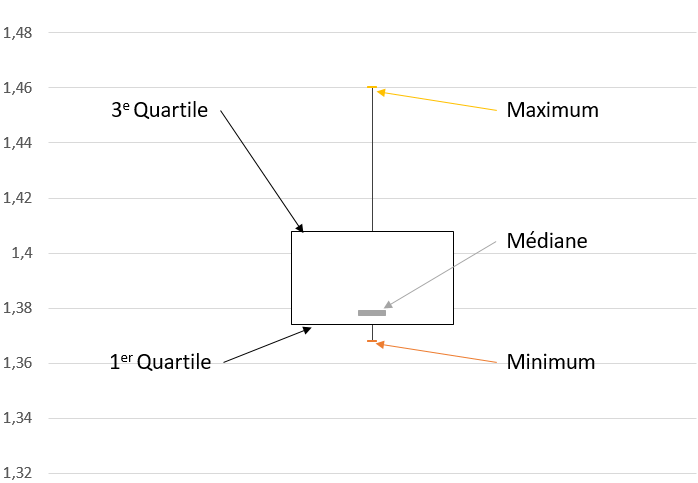
\includegraphics[scale=0.7]{moustache}
\end{center}
\end{document}